% Appendix
\chapter{How to use TAPS}
The required dependencies for generating the ANTLR4 parser, running TAPS and verification with FDR4 are listed below:
\begin{itemize}
    \item ANTLR4
    \item Python 2.7
    \item ANTLR Python runtime
    \item FDR4
\end{itemize}

ANTLR4 and FDR4 can both be downloaded from their websites, where installation instructions are also provided.
The ANTLR4 project can be found at \url{https://www.antlr.org/} and the FDR4 Project at \url{https://www.cs.ox.ac.uk/projects/fdr/}.\\
It is also necessary to download the ANTLR4 Python runtime from \url{https://pypi.org/project/antlr4-python2-runtime/}.
Assuming that an ANTLR4 alias has been created as the ANTLR4 installation suggest, the parser and lexer can be generated with ANTLR4 using the command: {\ttfamily antlr4 -Dlanguage=Python2 - visitor -no-listener Smeil.g4.}
This will create all the required parser and lexer files, as well as the visitor methods. This step is only necessary if the .g4 grammar file has been modified.\\

When the ANTLR4 files have been generated, TAPS can be used directly with a well-formed SMEIL program with the command: {\ttfamily python taps.py input.sme output.csp}. The system requires both an input file and an output file. If the output file does not exist, it will be created by TAPS. \\

The resulting \cspm{} file can be verified in FDR4, either by the command line tool or by the FDR4 tool, which is a graphical tool. The command line tool can be used by the command \texttt{refines output.csp}. There are several options to adjust the output of the command. The FDR4 command line tool is mostly used to quickly check if a network passes the verification, because it is difficult to navigate the counterexamples. The FDR4 graphical tool provides a better visualisation of counterexamples, and the ProBE visualiser can be called directly from the FDR4 graphical tool.

\chapter{Full SMEIL and \cspm code}
\begin{minted}{smeil_lexer.py:SMEILLexer -x}
proc clock ()
    bus clock_out {val: u17 range 1 to 86401;};
    var i: u17 = 0 range 0 to 86401;
{
    i = i + 1;
    clock_out.val = i;
}

proc hours (in hours_in)
    bus hours_out {first_digit: u2 range 0 to 2;
                   second_digit: u4 range 0 to 9;};
    var hours: u5 range 0 to 23;
    var hours_first_temp: u2 range 0 to 2;
    var hours_second_temp: u4 range 0 to 9;
{
    hours = hours_in.val / 3600 % 24;
    hours_first_temp = hours / 10;
    hours_second_temp = hours % 10;
    hours_out.first_digit = hours_first_temp;
    hours_out.second_digit = hours_second_temp;
}

proc minutes (in minutes_in)
    bus minutes_out {first_digit: u3 range 0 to 5;
                     second_digit: u4 range 0 to 9;};
    var minutes: u6 range 0 to 59;
    var minutes_first_temp: u3 range 0 to 5;
    var minutes_second_temp: u4 range 0 to 9;

{
    minutes = minutes_in.val / 60 % 60;
    minutes_first_temp = minutes / 10;
    minutes_second_temp = minutes % 10;
    minutes_out.first_digit = minutes_first_temp;
    minutes_out.second_digit = minutes_second_temp;
}


proc seconds (in seconds_in)
    bus seconds_out {first_digit: u3 range 0 to 5;
                     second_digit: u4 range 0 to 9;};
    var seconds: u6 range 0 to 59;
    var seconds_first_temp: u3 range 0 to 5;
    var seconds_second_temp: u4 range 0 to 9;
{
    seconds = seconds_in.val % 60;
    seconds_first_temp = seconds / 10;
    seconds_second_temp = seconds % 10;
    seconds_out.first_digit = seconds_first_temp;
    seconds_out.second_digit = seconds_second_temp;
}

network clock_network ()
{
    instance g of clock();
    instance h of hours(g.clock_out);
    instance m of minutes(g.clock_out);
    instance s of seconds(g.clock_out);
}

\end{minted}
\captionof{listing}{The full SMEIL code used for transpiling in the seven segment display example.\label{lst:smeil}}

\begin{minted}{cspm_lexer.py:CSPmLexer -x}
channel clock_out_val : {0..131071}

channel hours_out_first_digit : {0..3}
channel hours_out_second_digit : {0..15}

channel minutes_out_first_digit : {0..7}
channel minutes_out_second_digit : {0..15}

channel seconds_out_first_digit : {0..7}
channel seconds_out_second_digit : {0..15}


Hours(hours_in) =
let
    hours = hours_in / 3600  % 24
    hours_first_temp = hours / 10
    hours_second_temp = hours % 10
within
    hours_out_first_digit ! hours_first_temp ->
    hours_out_second_digit ! hours_second_temp ->
    SKIP

Hours_out_first_digit_monitor(c) =
    c ? x -> if 0 <= x and x <= 2 then SKIP else STOP
Hours_out_second_digit_monitor(c) =
    c ? x -> if 0 <= x and x <= 9 then SKIP else STOP


Minutes(minutes_in) =
let
    minutes = minutes_in / 60  % 60
    minutes_first_temp = minutes / 10
    minutes_second_temp = minutes % 10
within
    minutes_out_first_digit ! minutes_first_temp ->
    minutes_out_second_digit ! minutes_second_temp ->
    SKIP

Minutes_out_first_digit_monitor(c) =
    c ? x -> if 0 <= x and x <= 5 then SKIP else STOP
Minutes_out_second_digit_monitor(c) =
    c ? x -> if 0 <= x and x <= 9 then SKIP else STOP


Seconds(seconds_in) =
let
    seconds = seconds_in % 60
    seconds_first_temp = seconds / 10
    seconds_second_temp = seconds % 10
within
    seconds_out_first_digit ! seconds_first_temp ->
    seconds_out_second_digit ! seconds_second_temp ->
    SKIP

Seconds_out_first_digit_monitor(c) =
    c ? x -> if 0 <= x and x <= 5 then SKIP else STOP
Seconds_out_second_digit_monitor(c) =
    c ? x -> if 0 <= x and x <= 9 then SKIP else STOP


N_hours = clock_out_val ? variable ->
          (Hours(variable)
          [| {| hours_out_first_digit|} |]
          Hours_out_first_digit_monitor(hours_out_first_digit))
          [| {| hours_out_second_digit|} |]
          Hours_out_second_digit_monitor(hours_out_second_digit)

assert SKIP [F= N_hours \ Events


N_minutes = clock_out_val ? variable ->
            (Minutes(variable)
            [| {| minutes_out_first_digit|} |]
            Minutes_out_first_digit_monitor(minutes_out_first_digit))
            [| {| minutes_out_second_digit|} |]
            Minutes_out_second_digit_monitor(minutes_out_second_digit)

assert SKIP [F= N_minutes \ Events


N_seconds = clock_out_val ? variable ->
            (Seconds(variable)
            [| {| seconds_out_first_digit|} |]
            Seconds_out_first_digit_monitor(seconds_out_first_digit))
            [| {| seconds_out_second_digit|} |]
            Seconds_out_second_digit_monitor(seconds_out_second_digit)

assert SKIP [F= N_seconds \ Events

\end{minted}
\captionof{listing}{The full \cspm{} code after transpiling the seven segment display example, as seen in Listing~\ref{lst:smeil} in the appendix.\label{lst:cspm}}

\chapter{Towards Automatic Program Specification
Using SME Models}
\noindent A paper based on this thesis has been submitted for publication as

\begin{center}
\begin{minipage}{0.8\textwidth}
    A. Thegler, M. Larsen, K. Skovhede, and B. Vinter. "Towards automatic program specification using sme models". In: {\itshape Proceedings of Communicating Process Architectures
    2018} (2018)
\end{minipage}
\end{center}
The following pages contains this paper.
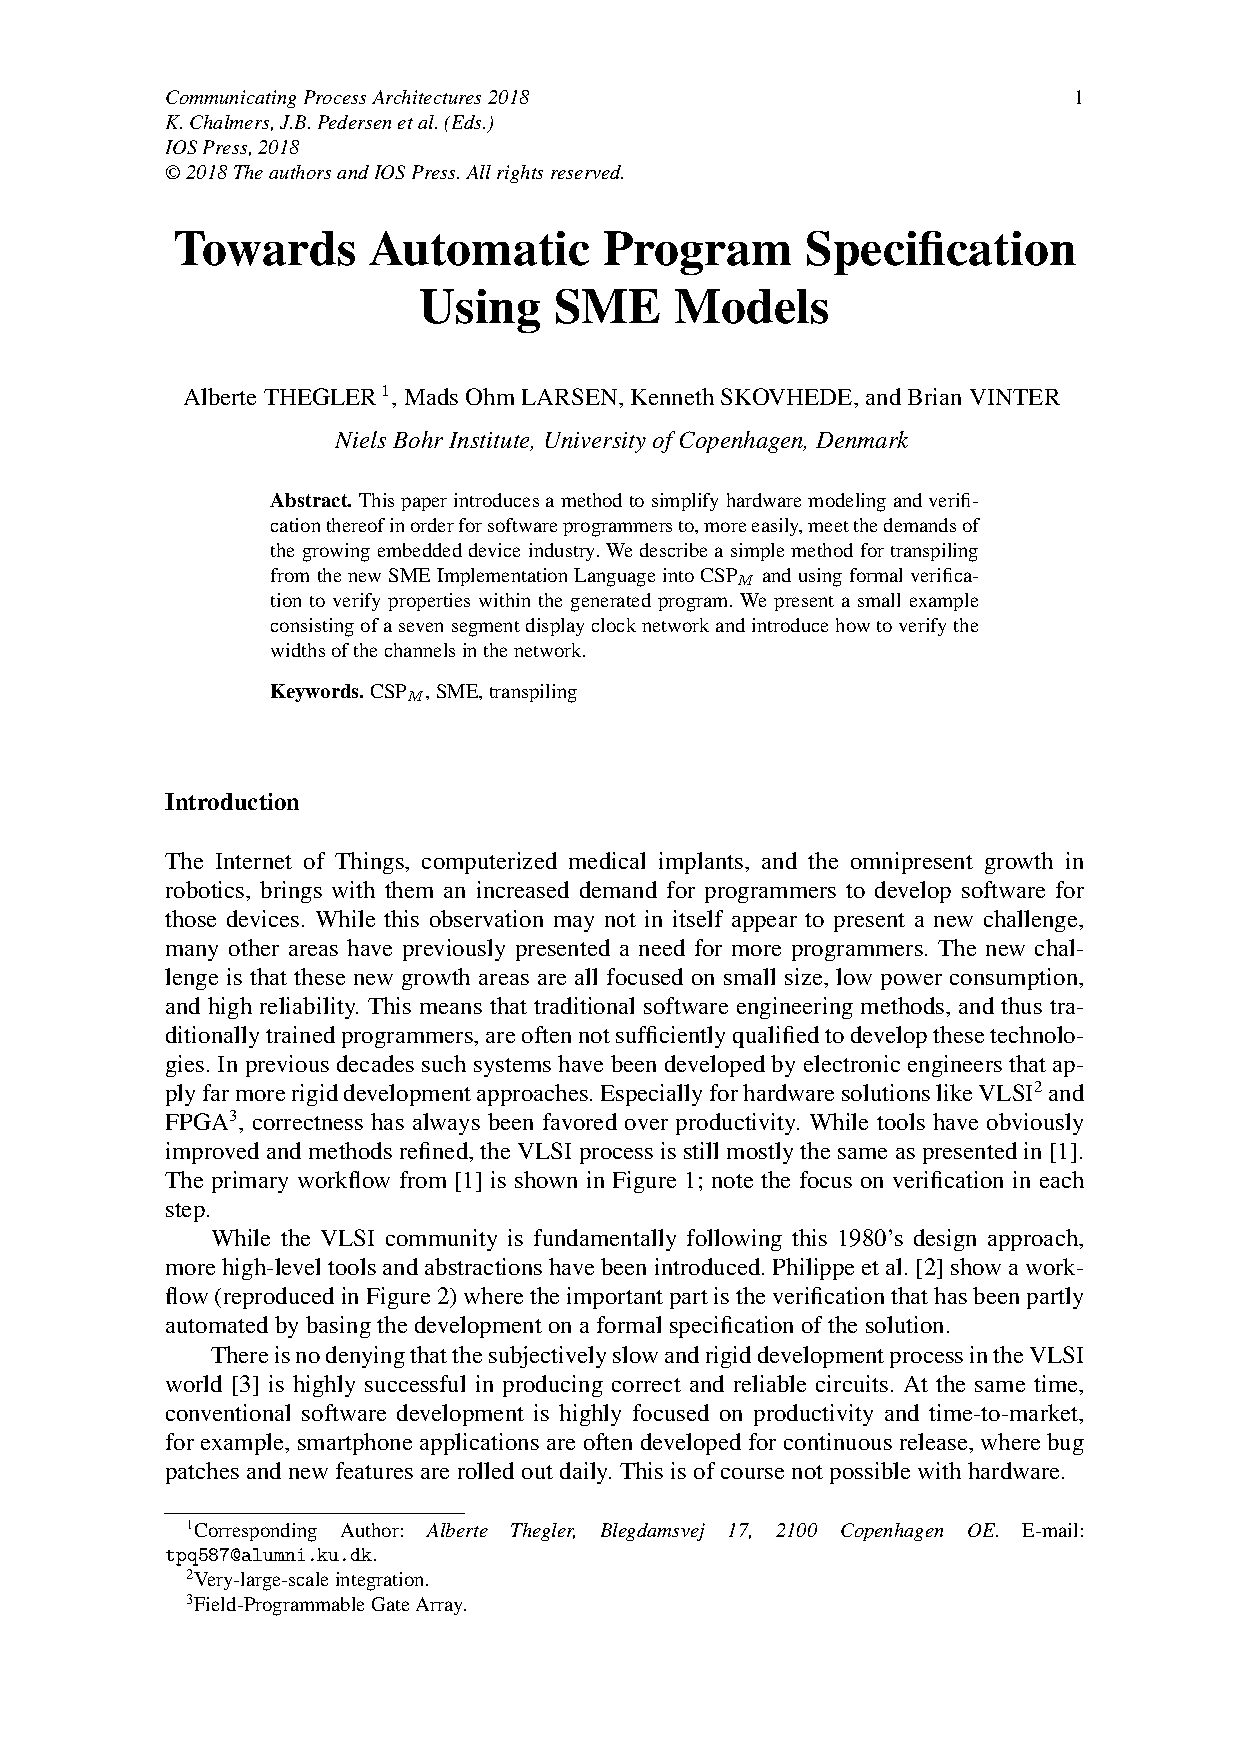
\includepdf[pages=-]{./paper/main.pdf}